\documentclass[11pt,a4paper]{article}

% ───────────────────────── Packages ─────────────────────────
\usepackage[T1]{fontenc}
\usepackage[margin=1in]{geometry}
\usepackage{lmodern}
\usepackage{graphicx}
\usepackage{xcolor}
\usepackage{booktabs}
\usepackage{longtable}
\usepackage{array}
\usepackage[hidelinks,colorlinks=true,linkcolor=navy,citecolor=navy,urlcolor=navy]{hyperref}
\usepackage{tikz}
\usetikzlibrary{shapes.geometric,arrows.meta,positioning,fit,backgrounds}
\usepackage{enumitem}
\usepackage{titlesec}
\usepackage{fancyhdr}
\usepackage{caption}
\usepackage{helvet}
\usepackage{tabularx}
\usepackage{setspace}
\usepackage{needspace}

% ───────────────────────── Colors ─────────────────────────
\definecolor{navy}{HTML}{00205B}
\definecolor{navydark}{HTML}{001438}
\definecolor{emerald}{HTML}{059669}
\definecolor{amber}{HTML}{B45309}
\definecolor{slate900}{HTML}{0F172A}
\definecolor{slate600}{HTML}{475569}
\definecolor{slate400}{HTML}{94A3B8}
\definecolor{slate100}{HTML}{F1F5F9}
\definecolor{slate50}{HTML}{F8FAFC}
\definecolor{bordergray}{HTML}{E2E8F0}

% ───────────────────────── Section styling ─────────────────────────
\titleformat{\section}
  {\normalfont\sffamily\Large\bfseries\color{navy}}
  {\thesection}{0.5em}{}[{\color{bordergray}\titlerule[1pt]}]
\titleformat{\subsection}
  {\normalfont\sffamily\large\bfseries\color{navy}}
  {\thesubsection}{0.5em}{}
\titleformat{\subsubsection}
  {\normalfont\sffamily\bfseries\color{slate900}}
  {\thesubsubsection}{0.5em}{}

\pagestyle{fancy}
\fancyhf{}
\renewcommand{\headrulewidth}{0.4pt}
\fancyhead[L]{\small\sffamily\color{slate600} PayerLens AI --- Project Report}
\fancyhead[R]{\small\sffamily\color{slate600} Novo Nordisk GBS Hackathon 2026}
\fancyfoot[C]{\small\sffamily\color{slate400} \thepage}

\setlength{\parskip}{0.55em}
\setlength{\parindent}{0pt}

\newcommand{\pill}[2]{%
  \tikz[baseline=-0.6ex]\node[fill=#1,rounded corners=2pt,inner sep=3pt,text=white,font=\sffamily\bfseries\scriptsize]{#2};%
}

% ───────────────────────── Document ─────────────────────────
\begin{document}

% ───────────────────────── Title page ─────────────────────────
\begin{titlepage}
\newgeometry{margin=0in}
\noindent
\colorbox{navy}{\parbox[c][3.2in][c]{\paperwidth}{
\hspace{1in}
\begin{minipage}{5.5in}
{\color{slate400}\sffamily\bfseries\small NOVO NORDISK GBS HACKATHON 2026}\\[0.35in]
{\color{white}\sffamily\bfseries\fontsize{34}{40}\selectfont PayerLens AI}\\[0.15in]
{\color{white!85!navy}\sffamily\Large Predicting Patient Access Through Payer \& \\Healthcare Ecosystem Intelligence}\\[0.3in]
{\color{white}\sffamily\itshape\normalsize Project Report}
\end{minipage}
}}

\vspace{0.6in}
\hspace{1in}
\begin{minipage}{5.5in}
\sffamily
{\color{slate400}\bfseries\small COLLEGE}\\
{\color{slate900}\large International Institute of Information Technology Bangalore}\\[0.25in]
{\color{slate400}\bfseries\small TEAM}\\
{\color{slate900}\Large Chamrajpet}\\[0.25in]
{\color{slate400}\bfseries\small TEAM MEMBERS}\\
{\color{slate600}\large Amogh Gurudatta, Surya Kiran Basava, Saaket Ajay Manjrekar, Kedar Mallya, Vamshidhar Vagish}\\[0.45in]
{\color{slate400}\bfseries\small LIVE DEPLOYMENT}\\
{\color{slate600}\normalsize
Frontend: \url{https://payer-lens-ai.vercel.app/}\\
Backend:\ \ \url{https://payerlens-ai-backend.onrender.com/}}
\end{minipage}

\vfill
\hspace{1in}
\begin{minipage}{5.5in}
\color{slate400}\sffamily\small
Global Health Economics \& Outcomes Research (HEOR) \& Market Access Intelligence Track
\end{minipage}
\vspace{0.5in}
\restoregeometry
\end{titlepage}

% ───────────────────────── Abstract ─────────────────────────
\begin{abstract}
\noindent
Manufacturers spend weeks of fragmented, manual health-economics analysis trying to anticipate how
divergent European Health Technology Assessment (HTA) bodies will respond to a new therapy.
\textbf{PayerLens AI} is an audit-ready web platform that simulates and predicts reimbursement
access probability for a heart-failure therapy across the United Kingdom (NICE), Germany
(G-BA/IQWiG), and France (HAS) --- combining a transparent, citation-backed multi-attribute
decision simulation with a calibrated machine-learning ensemble trained on 1,452 real and curated
historical HTA appraisal records. The platform lets a cross-functional team test price points,
companion-diagnostic requirements, and patient-population strategy against five real historical
drug precedents (Farxiga, Verquvo, Entresto, Jardiance, and a broad-class archetype), returning
country-specific access probabilities, budget-impact alerts, and a strategic launch-sequence
recommendation in real time. This report documents the problem motivating the platform, its
dual-engine system architecture, the data and modelling methodology (including a data-leakage
issue discovered and corrected during development), implementation and deployment details,
evaluation results, known limitations, and a roadmap toward production readiness.
\end{abstract}

% Force the ToC onto its own page — with the abstract above, its entries were
% previously being squeezed into the remaining space on that page and the
% last line ran past the bottom margin instead of wrapping to the next page.
\clearpage
\tableofcontents
\thispagestyle{fancy}
\newpage

% ═══════════════════════════════════════════════════════════
\section{Introduction}
% ═══════════════════════════════════════════════════════════

\subsection{Problem Statement}
Developing an innovative medicine is only the first step toward improving patient outcomes ---
the harder challenge begins after clinical success, when a manufacturer must decide how to achieve
timely reimbursement and broad patient access across fundamentally different healthcare systems.
Today, this strategic question is answered with fragmented analyses, historical experience, and
expert judgement, because healthcare ecosystems vary sharply across countries: payer expectations,
HTA frameworks, treatment pathways, and affordability thresholds all differ. A strategy that
succeeds in Germany may fail outright in the United Kingdom or France. No platform today lets a
manufacturer \emph{simulate} a country's healthcare ecosystem and predict how a given patient
population, evidence package, and market-access strategy will influence a real reimbursement
decision.

The specific business question this project addresses is drawn directly from the hackathon
problem statement: \emph{how can reimbursement be achieved for a new therapeutic category with a
unique mechanism of action for heart failure?} PayerLens AI is asked to identify the most
reimbursable patient segment and payer strategy by assessing cardiovascular risk, eligible patient
populations, and category-creation challenges, and to deliver a country-prioritized access
strategy --- including payer evidence needs and implementation requirements --- within four weeks.

\subsection{Motivation}
Three European HTA systems illustrate why this is hard:
\begin{itemize}[leftmargin=1.3em]
  \item \textbf{UK (NICE)} anchors decisions to a cost-utility ceiling of £20,000--£30,000 per
  QALY gained, plus a £20M national Budget Impact Test.
  \item \textbf{Germany (G-BA/IQWiG)}, under the AMNOG process (SGB V \S\,35a), legally
  \emph{forbids} cost-effectiveness (ICER) reasoning during benefit assessment and instead grades
  added clinical benefit (\emph{Zusatznutzen}) purely against a designated comparator.
  \item \textbf{France (HAS)} runs a dual track: \emph{SMR} (Service M\'edical Rendu) gates the
  reimbursement rate, while \emph{ASMR} (Amélioration du SMR, Level~I--V) gates the price premium
  CEPS will negotiate.
\end{itemize}
The same clinical evidence package can therefore be read three different ways by three different
statutory bodies. Building the intuition for this divergence today requires senior HEOR expertise
and weeks of cross-functional workshops between Market Access, Commercial, Regulatory, and Medical
Affairs teams.

\subsection{Objectives}
\begin{enumerate}[leftmargin=1.5em]
  \item Build an interactive simulation engine that predicts country-specific reimbursement access
  probability for a heart-failure therapy under user-defined price and evidence assumptions.
  \item Ground every prediction in real historical HTA precedent and make its provenance
  (statutory / clinical / epidemiological / simulated) explicit and auditable.
  \item Complement the transparent simulation with a calibrated machine-learning ensemble trained on
  genuine HTA appraisal outcomes, to test whether a data-driven approach agrees with, and can
  extend, expert-encoded heuristics.
  \item Package the result as a deployed, usable web application --- not a notebook --- so a
  cross-functional team can actually run scenarios live.
\end{enumerate}

% ═══════════════════════════════════════════════════════════
\section{Related Work and Existing Approaches}
% ═══════════════════════════════════════════════════════════
Health economics and outcomes research (HEOR) teams currently rely on a mix of (a) static,
manually-built Excel cost-effectiveness and budget-impact models built fresh for each submission,
(b) internal historical-precedent knowledge held by senior HEOR staff, and (c) commercial
market-access consultancy engagements that take weeks to turn around a country-prioritization
recommendation. None of these approaches are \emph{interactive} --- a change in target price or
trial design typically requires rebuilding the analysis from scratch --- and none systematically
tag every input to its statutory or clinical source in a way a payer-facing dossier could reuse
directly. Public HTA decision databases (e.g.\ France's \texttt{data.gouv.fr} ASMR/SMR registry)
exist but are not connected to any predictive or simulation layer. PayerLens AI's contribution is
to combine (i) a documented, citation-audited simulation engine with (ii) a calibrated ML model
trained directly on these public and curated statutory records, exposed through a single
interactive interface.

% ═══════════════════════════════════════════════════════════
\section{Proposed System}
% ═══════════════════════════════════════════════════════════

\subsection{Solution Overview}
PayerLens AI is an interactive dashboard that predicts the probability of reimbursement for a
heart-failure therapy across the UK, Germany, and France, letting a user test price points,
companion-diagnostic requirements, and patient-population strategy against five real historical
drug precedents: \textbf{Farxiga} (dapagliflozin, DAPA-HF biomarker-stratified archetype),
\textbf{Verquvo} (vericiguat, VICTORIA post-hospitalisation archetype), \textbf{Entresto}
(sacubitril/valsartan, PARADIGM-HF post-standard-of-care archetype), \textbf{Jardiance}
(empagliflozin, EMPEROR-Reduced severe-unmet-need archetype), and a \textbf{Broad Class}
unstratified-submission cautionary archetype.

\subsection{Key Features}
\begin{itemize}[leftmargin=1.3em]
  \item \textbf{Team Persona Bar} --- reframes the same underlying data for Market Access \&
  HEOR, Commercial \& Pricing, or Regulatory \& Medical Affairs perspectives.
  \item \textbf{Strategic Recommendation Engine} --- surfaces the optimal patient subgroup, a
  country launch sequence (e.g.\ Wave 1: Germany~$\to$~Wave 2: UK~$\to$~Wave 3: France), and
  critical evidence gaps for the active scenario.
  \item \textbf{Scenario controls} --- an annual acquisition price slider (\texteuro1,500--8,500)
  and a companion-diagnostic (NT-proBNP assay) toggle, both feeding the live simulation.
  \item \textbf{National HTA appraisal cards} --- one card per country showing simulated access
  probability, the decision currency that agency actually uses (ICER/QALY, \emph{Zusatznutzen},
  SMR/ASMR), and a budget-impact breach alert.
  \item \textbf{Comparative visualizations} --- active-scenario, cross-precedent, and
  price-sensitivity chart views plotted against a 70\% historical viability benchmark.
  \item \textbf{Clinical evidence \& commercial playbook} --- three linked cards covering the
  clinical trial evidence, likely payer objections, and the strategic response playbook.
  \item \textbf{Custom Molecule \& Trial Endpoint Simulator} --- lets a user define arbitrary
  trial endpoints and price, and run live ML inference with rule-based explainability
  (``decision drivers'': catalysts and frictions per jurisdiction).
  \item \textbf{Methodology and audit trail} --- a transparent derivation of every formula, and a
  slide-over dossier drawer with a full source bibliography.
  \item \textbf{Guided onboarding tour} for first-time users.
\end{itemize}

\subsection{Target Users and Use Case}
The primary user is a \textbf{Market Access / HEOR analyst} preparing a pre-launch access strategy
for a novel-mechanism heart-failure therapy. A representative use case: \emph{``Given our Phase~3
trial data and a target price, which country should we launch in first, and what evidence gap must
we close before submission?''} Secondary users include Commercial/Pricing (price-elasticity
war-gaming) and Regulatory/Medical Affairs (aligning trial design with payer evidence
requirements).

% ═══════════════════════════════════════════════════════════
\section{System Architecture}
% ═══════════════════════════════════════════════════════════

\subsection{High-Level Architecture}
The system separates an \emph{offline training pipeline} from a \emph{live request/response path},
with the frontend able to degrade gracefully to a local heuristic when the ML service is
unreachable. Figure~\ref{fig:architecture} summarises the design.

\begin{figure}[h]
\centering
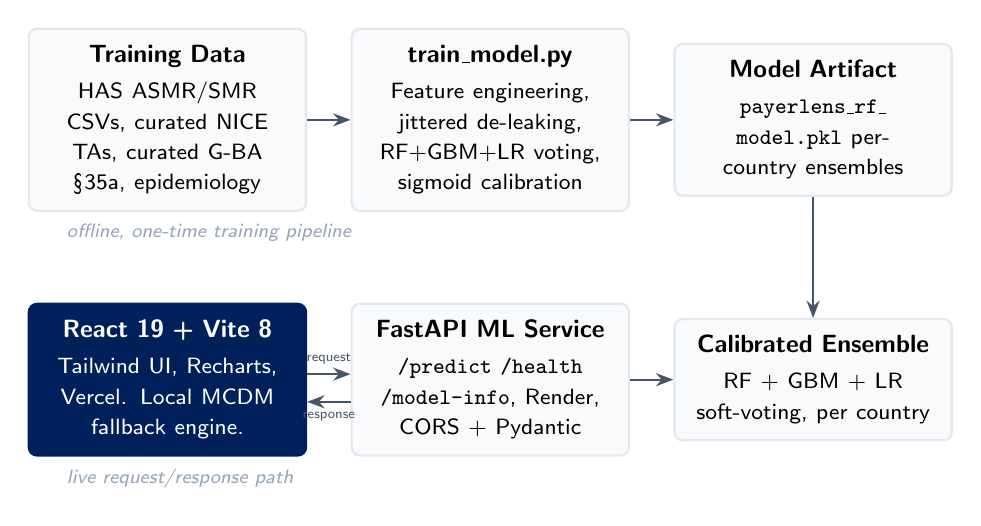
\begin{tikzpicture}[
  box/.style={draw=bordergray, thick, rounded corners=3pt, fill=slate50, align=center,
              minimum height=1.3cm, font=\sffamily\small, text width=3.1cm, inner sep=6pt},
  navybox/.style={box, fill=navy, draw=navy, text=white},
  arr/.style={-{Stealth[length=2.2mm]}, thick, color=slate600},
  lbl/.style={font=\sffamily\scriptsize\itshape, color=slate400}
]
% offline row
\node[box] (data) at (0,4) {\textbf{Training Data}\\[2pt]\footnotesize HAS ASMR/SMR CSVs, curated NICE TAs, curated G-BA \S35a, epidemiology};
\node[box] (train) at (4.1,4) {\textbf{train\_model.py}\\[2pt]\footnotesize Feature engineering, jittered de-leaking, RF+GBM+LR voting, sigmoid calibration};
\node[box] (artifact) at (8.2,4) {\textbf{Model Artifact}\\[2pt]\footnotesize \texttt{payerlens\_rf\_\allowbreak model.pkl} per-country ensembles};
\draw[arr] (data) -- (train);
\draw[arr] (train) -- (artifact);
\node[lbl, below=1pt of data, anchor=north west, xshift=-1.4cm] {offline, one-time training pipeline};

% runtime row
\node[navybox] (fe) at (0,0.7) {\textbf{React 19 + Vite 8}\\[2pt]\footnotesize Tailwind UI, Recharts, Vercel. Local MCDM fallback engine.};
\node[box] (api) at (4.1,0.7) {\textbf{FastAPI ML Service}\\[2pt]\footnotesize \texttt{/predict /health /model-info}, Render, CORS + Pydantic};
\node[box] (ens) at (8.2,0.7) {\textbf{Calibrated Ensemble}\\[2pt]\footnotesize RF + GBM + LR soft-voting, per country};
\draw[arr] ([yshift=2pt]fe.east) -- ([yshift=2pt]api.west) node[midway, above, font=\tiny\sffamily] {request};
\draw[arr] ([yshift=-8pt]api.west) -- ([yshift=-8pt]fe.east) node[midway, below, font=\tiny\sffamily] {response};
\draw[arr] (api) -- (ens);
\draw[arr] (artifact) -- (ens);
\node[lbl, below=1pt of fe, anchor=north west, xshift=-1.4cm] {live request/response path};
\end{tikzpicture}
\caption{PayerLens AI dual-path architecture: an offline model-training pipeline feeds a
versioned artifact into a FastAPI inference service, while the React frontend calls that service
live (falling back to a local calibrated heuristic engine if it is unreachable). When the live
service is reachable, its prediction --- not the local fallback --- is what the dashboard shows.}
\label{fig:architecture}
\end{figure}

\subsection{Data Flow}
\begin{enumerate}[leftmargin=1.5em]
  \item A user selects a historical precedent scenario and adjusts price / diagnostic assumptions
  in the browser.
  \item The frontend derives ML-ready features (e.g.\ an ICER band and a cost-ratio-to-SoC from
  the chosen price) and calls \texttt{POST /predict} on the FastAPI service.
  \item The service selects the country-specific calibrated ensemble, returns access probabilities,
  a composite score, class probabilities, and rule-based decision drivers.
  \item The frontend layers a documented, additive companion-diagnostic friction penalty on top of
  the live model output (a regulatory delay effect the model was not trained to detect) and renders
  the country cards, charts, and recommendation banner.
  \item If the API call fails (e.g.\ a cold-started free-tier backend), the frontend instead
  computes the same country scores from a local, fully documented multi-attribute decision
  formula, so the application never blocks on network availability.
\end{enumerate}

% ═══════════════════════════════════════════════════════════
\section{Methodology}
% ═══════════════════════════════════════════════════════════

\subsection{Data Sources and Provenance}
The training corpus merges three sources into 1,452 labelled records:
\begin{itemize}[leftmargin=1.3em]
  \item \textbf{France (HAS), 1,337 records} --- parsed directly from the live ASMR and SMR CSV
  registries published on \texttt{data.gouv.fr} (Commission de la Transparence), restricted to
  \emph{inscription} / \emph{renouvellement} motifs with a valid ASMR grade (I--V), with the
  over-represented ASMR-V class capped at 350 rows to reduce class imbalance.
  \item \textbf{United Kingdom (NICE), 73 records} --- hand-curated from real NICE Technology
  Appraisal outcomes (e.g.\ TA388, TA665, TA773, TA793) spanning heart failure and adjacent
  cardiometabolic and oncology indications, to give the UK model enough label diversity.
  \item \textbf{Germany (G-BA), 42 records} --- hand-curated from real \S\,35a AMNOG benefit
  resolutions.
\end{itemize}
Every record also carries a \textbf{provenance tag} --- \emph{Statutory}, \emph{Clinical},
\emph{Epidemiological}, or \emph{Simulated} --- surfaced in the UI so a reviewer can distinguish a
directly-cited statutory ruling from a calibrated estimate.

\subsection{Feature Engineering}
Thirteen features describe each record: ICER band, direct-comparator flag, mortality hazard
ratio, hospitalisation reduction, biomarker-defined flag, budget impact, unmet-need rating,
orphan-drug status, quality-of-life improvement, evidence grade, pre-specified-subgroup flag,
safety/tolerability rating, and cost ratio versus standard of care. For the France corpus, most
records only have a drug name and its ASMR/SMR outcome (not a full clinical feature set), so the
remaining features are imputed from an ASMR-level lookup table calibrated to HAS doctrine.

\subsection{Addressing a Data-Leakage Issue}
\label{sec:leakage}
During evaluation of the first trained model, a methodological issue was identified: the ASMR-level
lookup table used to impute features for unmatched French drugs produced a \emph{deterministic},
one-to-one mapping from a drug's ASMR grade to its feature vector --- and the training label was
itself derived from that same ASMR grade. Concretely, every drug placed in ASMR bucket ``IV''
received the exact same hazard ratio, hospitalisation reduction, safety score, and cost ratio,
regardless of what the drug actually was. A classifier can trivially exploit this by learning to
decode the ASMR bucket back out of the feature vector, which had it re-deriving its own label
rather than learning a genuine feature-to-outcome relationship, artificially inflating
cross-validated accuracy in a way that would not generalise to a genuinely new molecule (where the
ASMR grade is precisely the unknown quantity being predicted).

\textbf{Fix.} Each imputed feature is now sampled from a distribution centred on its ASMR-level
default with realistic relative noise (continuous features via multiplicative jitter, integer
features rounded after jitter and clipped to their valid range, and two binary flags --- direct
comparator and pre-specified subgroup --- randomly flipped with small probability). This converts
an exact, perfectly invertible mapping into a genuinely noisy correlation, which is what a
real-world relationship between trial evidence and appraisal outcome should look like. The model
was retrained after this fix; Section~\ref{sec:results} reports the corrected, more honest
accuracy figures. A related bug in the same training script --- the number of stratified
cross-validation folds was computed from the \emph{full} dataset's class counts rather than the
post-train/test-split counts, which could make a small class fail probability calibration silently
--- was fixed at the same time by deriving the fold count from the post-split training labels.

\subsection{Model Training}
For each country, a \textbf{soft-voting ensemble} of a Random Forest, a Gradient Boosting
classifier, and a class-balanced Logistic Regression is trained, then wrapped in
\texttt{CalibratedClassifierCV} with sigmoid (Platt) calibration so the output behaves as a
genuine probability rather than an uncalibrated classifier score. Cross-validation uses
\texttt{StratifiedKFold} with a fold count bounded by the smallest class size in the training
split. An 80/20 train/test split (stratified where class counts allow) is held out per country for
the accuracy figures reported in Section~\ref{sec:results}. A combined, all-country fallback model
is trained the same way for use when no country-specific model is available (e.g.\ an older
artifact format).

\subsection{The Local MCDM Simulation Engine}
Independently of the ML model, a documented multi-criteria decision formula computes each
country's access probability as a calibrated base probability (per historical precedent scenario)
plus price-sensitivity and companion-diagnostic modifiers specific to that country's statutory
character --- e.g.\ the UK modifier scales steeply above a €4,200/year baseline reflecting the
ICER ceiling, while Germany's modifier reflects AMNOG arbitration risk above a higher
\texteuro5,500 threshold. This engine has no dependency on the ML backend, and is what the frontend
falls back to only when the ML API is unreachable --- whenever the live service responds, its
prediction is what the application actually displays (see Section~\ref{sec:results} and
Figure~\ref{fig:architecture}).

% ═══════════════════════════════════════════════════════════
\section{Implementation}
% ═══════════════════════════════════════════════════════════

\subsection{Frontend}
The client is a React~19 single-page application built with Vite~8 and styled with Tailwind CSS,
using Recharts for the comparative visualizations and \texttt{react-joyride} for the guided
onboarding tour. State (selected scenario, price, diagnostic toggle, active modal) is held in the
root \texttt{App} component; a debounced effect re-queries the ML backend as price changes so the
live prediction stays responsive to the slider without spamming the API on every pixel of drag.

\subsection{Backend}
The inference service is a FastAPI application exposing three endpoints:
\begin{itemize}[leftmargin=1.3em]
  \item \texttt{GET /health} --- service and model-version status.
  \item \texttt{GET /model-info} --- feature list, per-country accuracies, and feature
  importances, so the frontend can display the model's \emph{real} measured accuracy instead of a
  hard-coded figure.
  \item \texttt{POST /predict} --- accepts a Pydantic-validated feature payload (optionally scoped
  to a single \texttt{country}), and returns per-country access probabilities, a composite score,
  per-class probabilities, and rule-based decision-driver explainability.
\end{itemize}

\subsection{Deployment}
The frontend is deployed on \textbf{Vercel} at
\url{https://payer-lens-ai.vercel.app/}, and the FastAPI backend on \textbf{Render} at
\url{https://payerlens-ai-backend.onrender.com/}, with the frontend's API base URL configured via
a build-time environment variable so the same codebase can target a local backend during
development.

% ═══════════════════════════════════════════════════════════
\section{Results and Evaluation}
\label{sec:results}
% ═══════════════════════════════════════════════════════════

\subsection{Model Performance}
Table~\ref{tab:accuracy} reports held-out test accuracy per country after the data-leakage fix
described in Section~\ref{sec:leakage}.

\begin{table}[h]
\centering
\begin{tabularx}{\textwidth}{@{}l r r X@{}}
\toprule
\textbf{Model} & \textbf{Training rows} & \textbf{Test acc.} & \textbf{Notes} \\
\midrule
UK (NICE) & 73 & 73.3\% & Small hand-curated corpus \\
Germany (G-BA) & 42 & 88.9\% & Small hand-curated corpus \\
France (HAS) & 1,337 & 94.8\% & Large corpus; residual label/ASMR correlation (\S\ref{sec:leakage}) \\
Combined (fallback) & 1,452 & 82.8\% & All countries pooled \\
\bottomrule
\end{tabularx}
\caption{Held-out test accuracy by country-specific model, after the jittering fix.}
\label{tab:accuracy}
\end{table}

France's accuracy remains high even after removing the deterministic leakage, because its label
and its (now merely noisy, not exact) features still both trace back to the same underlying ASMR
grade --- a structural property of the source data, not a remaining bug. Closing this gap fully
would require independent, per-drug trial-level features that are not present in the public
ASMR/SMR registry (see Section~\ref{sec:roadmap}).

\subsection{Example Walkthrough}
Table~\ref{tab:walkthrough} shows a concrete input/output example from the live, deployed system
for Scenario~D (the Farxiga / DAPA-HF biomarker-stratified archetype) at two price points, with the
companion diagnostic required in both cases.

\begin{table}[h]
\centering
\begin{tabular}{lcccc}
\toprule
\textbf{Price} & \textbf{UK} & \textbf{Germany} & \textbf{France} & \textbf{EU-3 composite} \\
\midrule
\texteuro4,200 (baseline) & 72\% & 80\% & 92\% & 81\% (Viable) \\
\texteuro8,500 (ceiling)  & 40\% & 60\% & 84\% & 61\% (High friction) \\
\bottomrule
\end{tabular}
\caption{Live model output for Scenario D (HR 0.68, 32\% hospitalisation reduction,
biomarker-defined, direct comparator) at two price points.}
\label{tab:walkthrough}
\end{table}

\subsection{User Interface}
Figure~\ref{fig:dashboard} shows the main dashboard for this scenario; Figure~\ref{fig:chart}
shows the cross-precedent comparison view; Figure~\ref{fig:simulator} shows the Custom Molecule
Simulator returning a live prediction with jurisdiction-level decision drivers.

\begin{figure}[h]
\centering
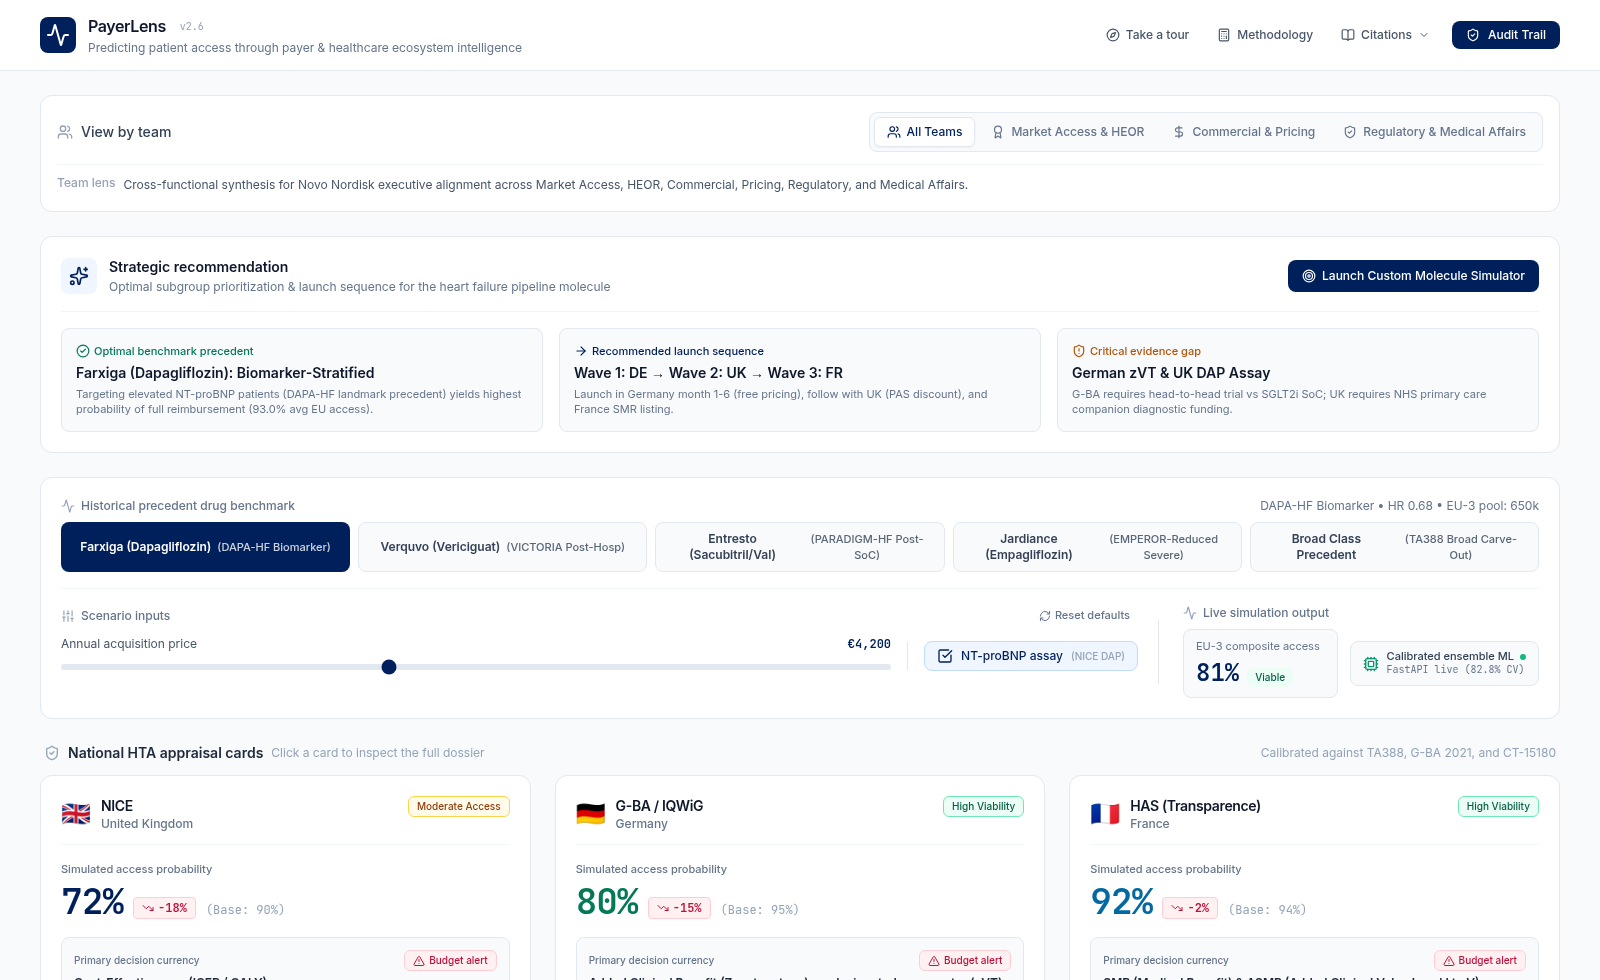
\includegraphics[width=\textwidth]{figures/report-hero.png}
\caption{PayerLens AI dashboard --- team persona bar, strategic recommendation, historical
precedent selector, scenario controls, and national HTA appraisal cards.}
\label{fig:dashboard}
\end{figure}

\begin{figure}[h]
\centering
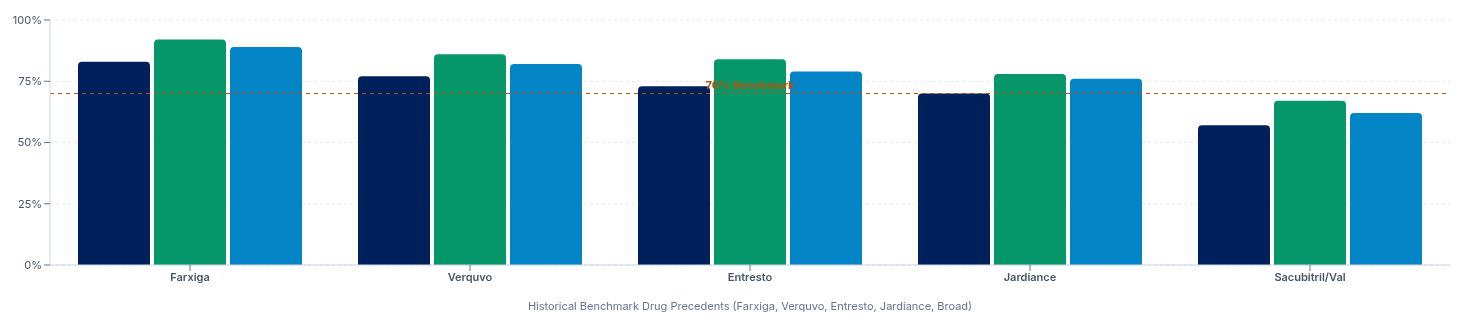
\includegraphics[width=\textwidth]{figures/report-chart-precedents.png}
\caption{Cross-precedent comparison: simulated access probability for all five historical drug
archetypes against the 70\% historical viability benchmark (dashed line).}
\label{fig:chart}
\end{figure}

\begin{figure}[h]
\centering
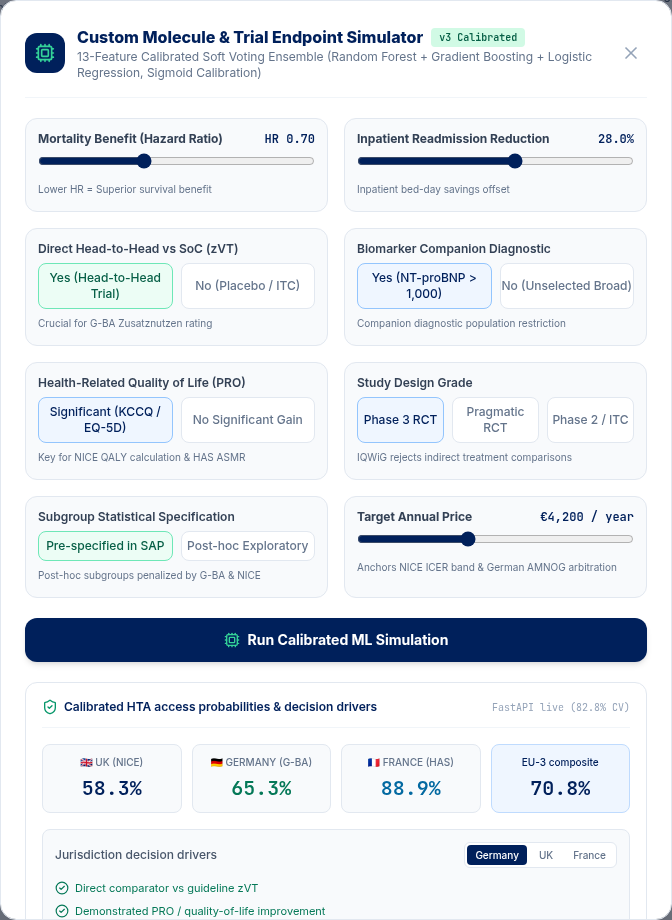
\includegraphics[width=0.62\textwidth]{figures/report-simulator.png}
\caption{Custom Molecule \& Trial Endpoint Simulator: a user-defined scenario returns live,
calibrated access probabilities and rule-based jurisdiction decision drivers.}
\label{fig:simulator}
\end{figure}

\subsection{Limitations Discovered}
\begin{itemize}[leftmargin=1.3em]
  \item The France dataset's structural label/feature correlation (Section~\ref{sec:leakage})
  bounds how far accuracy can be trusted as a proxy for generalisation to a genuinely novel
  molecule.
  \item The UK and Germany models train on comparatively small, hand-curated corpora (73 and 42
  rows), so their accuracy estimates carry more sampling variance than France's.
  \item The ML model has no native feature for companion-diagnostic requirements; this is
  currently applied as a documented additive penalty on top of the model's output rather than a
  learned interaction.
  \item Render's free hosting tier sleeps the backend after inactivity, so the first live request
  after a period of idleness can take up to roughly a minute, during which the frontend correctly
  falls back to its local heuristic.
\end{itemize}

% ═══════════════════════════════════════════════════════════
\section{Feasibility and Roadmap}
\label{sec:roadmap}
% ═══════════════════════════════════════════════════════════

\subsection{Feasible Next Steps}
Closing the France data-circularity gap with independent, per-drug trial-level features (e.g.\
extracted from EPAR or ClinicalTrials.gov endpoints rather than imputed from the ASMR grade)
is the highest-value next step, followed by expanding to the remaining EU-5 markets named in the
original problem statement (Italy's AIFA and Spain's AEMPS) and replacing rule-based
explainability with SHAP-based explainability computed directly from the trained ensemble.

\subsection{Roadmap}
\begin{enumerate}[leftmargin=1.5em]
  \item[\textbf{M1}] \textbf{Independent feature pipeline} --- source real per-drug trial
  features to replace the remaining imputed France features.
  \item[\textbf{M2}] \textbf{EU-5 expansion} --- add Italy (AIFA) and Spain (AEMPS) HTA models.
  \item[\textbf{M3}] \textbf{Native explainability} --- SHAP-based feature attribution from the
  trained ensemble, replacing the current rule-based decision drivers.
  \item[\textbf{M4}] \textbf{Enterprise readiness} --- authentication, persisted scenario
  libraries, and audit logging for compliance sign-off.
\end{enumerate}

\subsection{Dependencies and Risks}
\begin{itemize}[leftmargin=1.3em]
  \item Stability of the public \texttt{data.gouv.fr} schema and resource URLs the training
  pipeline depends on.
  \item Availability and licensing of NICE/G-BA appraisal data at a scale beyond hand curation.
  \item Model generalisation to therapeutic areas outside cardiology.
  \item Render's free-tier cold-start latency affecting live-demo reliability.
\end{itemize}

\subsection{Mitigation Plan}
\begin{itemize}[leftmargin=1.3em]
  \item The local calibrated MCDM engine keeps the application fully usable even if the ML
  service is unreachable.
  \item The model artifact is versioned, and \texttt{/model-info} reports its real measured
  accuracy so the UI never claims a stale or invented figure.
  \item The jittered-imputation methodology (Section~\ref{sec:leakage}) is documented for audit
  reproducibility.
\end{itemize}

% ═══════════════════════════════════════════════════════════
\section{Business Impact and Value Proposition}
% ═══════════════════════════════════════════════════════════

\subsection{Value Proposition}
PayerLens AI directly answers the hackathon problem statement's mandate: deliver a
country-prioritized access strategy --- including payer evidence needs and implementation
requirements --- within four weeks. It replaces fragmented, multi-week manual HEOR analysis with a
live, evidence-cited simulation that a cross-functional team can run interactively in a single
meeting.

\subsection{Adoption Pathway}
A realistic rollout starts with a \textbf{pilot} on the current heart-failure scope, followed by
\textbf{cross-functional validation} with Market Access, HEOR, Regulatory, and Commercial
stakeholders, then \textbf{expansion} to the remaining EU-5 markets and additional indications, and
finally \textbf{embedding} the tool into the enterprise launch-planning workflow.

\subsection{Evidence and Assumptions}
The simulation is calibrated against real historical HTA rulings (NICE TA388/679/773/793, G-BA
benefit resolutions, HAS Commission de la Transparence opinions). It explicitly \emph{assumes} that
payer behaviour toward a new-mechanism heart-failure therapy will pattern-match these historical
precedents --- stated here as an assumption, not a guarantee, and the tool is positioned to
\emph{augment}, not replace, HEOR expert judgement.

\subsection{Key Takeaways}
\begin{enumerate}[leftmargin=1.5em]
  \item One platform replaces weeks of fragmented manual analysis with a live, interactive
  simulation.
  \item Every prediction is citation-backed and audit-ready --- not a black box.
  \item A dual transparent-simulation-plus-calibrated-ML design balances explainability with
  predictive power.
\end{enumerate}

% ═══════════════════════════════════════════════════════════
\section{Conclusion}
% ═══════════════════════════════════════════════════════════
PayerLens AI demonstrates that a market-access strategy question --- historically answered through
weeks of fragmented, manual HEOR analysis --- can be reframed as an interactive simulation grounded
in real regulatory precedent. The project's dual-engine design, pairing a transparent,
citation-audited decision model with a calibrated machine-learning ensemble, gives both
explainability and predictive power, while a documented local fallback keeps the tool usable
regardless of backend availability. Equally important to the platform itself was the process of
auditing it: a genuine data-leakage issue was found in the training pipeline and corrected,
producing a more honest (lower, but trustworthy) accuracy figure --- a result we view as a feature
of rigorous engineering practice, not a setback. The identified roadmap --- independent trial-level
features, EU-5 expansion, native explainability, and enterprise readiness --- defines a credible
path from hackathon prototype to a tool a real Market Access team could rely on.

% ═══════════════════════════════════════════════════════════
\section*{References}
\addcontentsline{toc}{section}{References}
% ═══════════════════════════════════════════════════════════
\begin{enumerate}[leftmargin=1.5em,label={[\arabic*]}]
\small
\item National Institute for Health and Care Excellence (NICE). \emph{Health Technology
Evaluations: The Manual} (PMG36), 2022.
\item NICE Technology Appraisal Guidance TA388: \emph{Sacubitril valsartan for treating
symptomatic chronic heart failure with reduced ejection fraction}, 2016.
\item NICE Technology Appraisal Guidance TA679, TA773, TA793 (dapagliflozin, empagliflozin,
vericiguat in heart failure).
\item Gemeinsamer Bundesausschuss (G-BA). Benefit assessment resolutions under \S\,35a SGB~V
(AMNOG), various years.
\item Haute Autorité de Santé (HAS), Commission de la Transparence. \emph{Doctrine for the
Evaluation of Medicinal Products}, 2020, and individual ASMR/SMR opinions (data.gouv.fr).
\item McMurray, J.J.V.\ et al. \emph{Dapagliflozin in Patients with Heart Failure and Reduced
Ejection Fraction} (DAPA-HF). \emph{N Engl J Med} 2019;381:1995--2008.
\item McMurray, J.J.V.\ et al. \emph{Angiotensin--Neprilysin Inhibition versus Enalapril in Heart
Failure} (PARADIGM-HF). \emph{N Engl J Med} 2014;371:993--1004.
\item Packer, M.\ et al. \emph{Cardiovascular and Renal Outcomes with Empagliflozin in Heart
Failure} (EMPEROR-Reduced). \emph{N Engl J Med} 2020;383:1413--1424.
\item Armstrong, P.W.\ et al. \emph{Vericiguat in Patients with Heart Failure and Reduced Ejection
Fraction} (VICTORIA). \emph{N Engl J Med} 2020;382:1883--1893.
\item European Society of Cardiology. \emph{2021 ESC Guidelines for the Diagnosis and Treatment of
Acute and Chronic Heart Failure}. \emph{Eur Heart J} 2021;42(36):3599--3726.
\item NHS Digital. \emph{Hospital Episode Statistics --- Admitted Patient Care}, 2022--2023.
\item British Heart Foundation. \emph{Heart \& Circulatory Disease Statistics}, 2024.
\end{enumerate}

\end{document}
